\documentclass[a4paper,11pt]{article} %, landscape report

\usepackage[T1]{fontenc}
\usepackage[utf8x]{inputenc}

%Selon les goûts: times palatino bookman newcent chancery helvet avant fourier kpfonts cmbright
%\usepackage{avant}

%\usepackage[hmargin=2cm,vmargin=2cm]{geometry}
%\usepackage{multicol}
%\setlength{\columnsep}{1cm}

\usepackage{graphicx}
\usepackage{xcolor}
\usepackage{multicol}\setlength{\columnsep}{1cm}

\usepackage{amsmath,amssymb,amsfonts,makeidx}
\usepackage{stmaryrd}% crochets «intervalles d'entiers»
%\newcommand{\B}{\mathbb{B}}
\usepackage{tikz}

\usepackage{lscape}

\newcommand{\vesp}{\vspace*{0.2em}}
\newcommand{\VESP}{\vspace*{0.8em}}
\newcommand{\ttt}[1]{\texttt{#1}}
\newcommand{\code}[1]{\colorbox{gray!15}{\texttt{#1}}}


\usepackage{hyperref}
\hypersetup{colorlinks=true, 
            linkcolor=violet,
            urlcolor=teal,
            citecolor=olive,
            }
\newcommand{\www}[2]{\href{#1}{\nolinkurl{#2}}}
%black, blue, brown, cyan, darkgray, gray, green, lightgray, lime, magenta, olive, orange, pink, purple, red, teal, violet, white, yellow
%\urlstyle{same}% Pas stylés \og URL

%\usepackage[nosort]{cite}

%\newcommand{\1}{\textcircled{\small 1}}
%\newcommand{\2}{\textcircled{\small 2}}
\setlength{\parskip}{0.2em}
%\setlength{\parindent}{0ex}

\usepackage[french]{babel} \frenchbsetup{StandardLists=true}
\usepackage[autolanguage]{numprint}
\DecimalMathComma

\AddThinSpaceBeforeFootnotes
\FrenchFootnotes

% =================================================================================================
%\title{Projet d'initiation à la Recherche\\M2 I2A}
%\author{Jean-Marc Gervais\\[0.6em]
%Encadré par M. Jean-François Couchot\\
%\small Institut FEMTO-ST, UMR 6174 CNRS -- DISC Équipe AND}
%\date{$15$ janvier $2\,020$}

\begin{document}%\setlength\parindent{5mm}
%\maketitle
%%
%\section*{\center Notes...\\[1cm]pytorch-dp}
%%
%\thispagestyle{empty}
%\newpage
%%
%\tableofcontents
%\newpage
\section{Deep Learning}
\emph{\textbf{Faut-il en donner le principe (neurone artificiel, couches, back-propagation / (S)GD) ??}}
\section{Réseaux de neurones convolutifs -- CNN}
\emph{\textbf{Idem: faut-il les présenter ?}}
\section{Exemple avec MNIST}
On présente ici l'architecture choisie pour l'exemple inclus dans \ttt{mnist.py}, d'abord sans se préoccuper de préservation de la confidentialité. La structure associée est celle de la classe \ttt{SampleConvNet} qui hérite de \ttt{nn.Module} où \ttt{nn} est l'alias habituel pour \ttt{torch.nn}, qui sert de base aux divers réseaux neuronaux dans \textsf{PyTorch}.

Chacune des entrées du lot traité sera une image en niveaux de gris de $28\times28$ pixels (qui sera au préalable normalisée). Le constructeur crée deux couches convolutives, suivies d'une couche classique \emph{fully connected} qui aboutit en sortie aux $10$ neurones associés à chacun des chiffres à identifier. La méthode \ttt{forward()} qui s'exécutera à chaque \emph{epoch}, autrement dit à chaque itération du processus d'apprentissage, définit les transformations pour passer d'une couche à la suivante: 
\begin{itemize}
	\item 
	Chaque image du \emph{batch} est transformée par convolution avec un \emph{kernel} (un filtre) de dimension $8\times8$ et qui parcours l'image par pas de $2$ (\emph{stride}) suivant chacune de ses dimensions, sans utiliser de \emph{padding}. Il a une profondeur de $16$ (il a $16$ \emph{channels}), et produit donc en sortie une couche de $11\times11$\footnote{Voir les explications sur le schéma général. Idem pour les dimensions suivantes} de profondeur $16$.
	\item 
	En sortie, la non-linéarité est assurée par la fonction ReLU (\emph{Rectified Linear Unit}) qui se réduit à l'identité sur l'ensemble des positifs et à la fonction nulle pour les négatifs. Les valeurs sont alors sous-échantillonnées par un \og max-\emph{pooling}\fg{} de $2\times2$, d'où les dimensions $10\times10$ en sortie. 
	\item 
	La seconde convolution est associée à un \emph{kernel} de $4\times4$ et de profondeur $32$, appliqué par pas de $2$ sans \emph{padding}, d'où la dimension $4\times4$ de la couche suivante.
	\item 
	Cette dernière subit à nouveau un max-\emph{pooling} $2\times2$ sans \emph{padding}, pour arriver un des données en $3\times3$ de profondeur $32$. 
	\item 
	Ces données sont remises \og à plat\fg{} sous forme d'un vecteur de taille $32\times3\times3$. Ce dernier est enfin relié aux $10$ neurones de la couche visible de sortie, en mode \emph{fully connected} comme dans un réseau de neurone basique. 
\end{itemize}
Là, on détaille comment le faire fonctionner uniquement ?

+ Principe intéressant de PyTorch = autograd
\begin{landscape}
	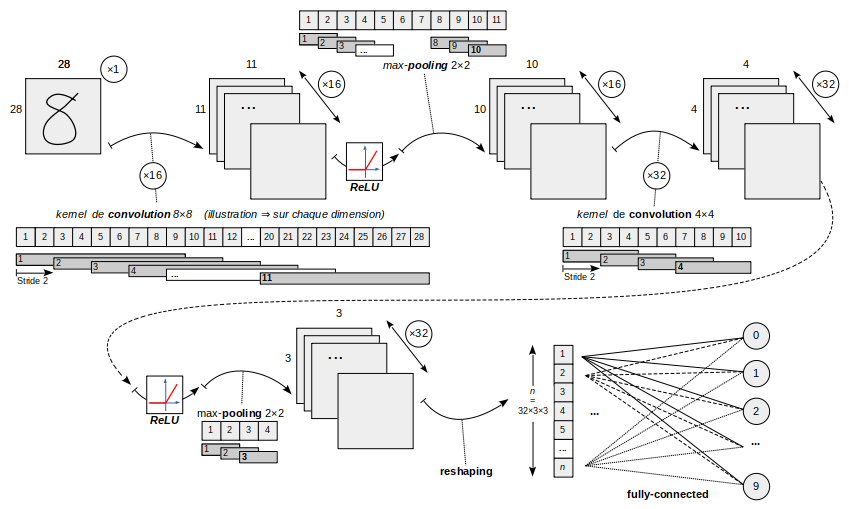
\includegraphics[width=\linewidth]{cnn.png}
\end{landscape}
\section{Ajout de confidentialité différentielle dans \ttt{mnist.py}}
Etc.

\section{Exploration de \texttt{pytorch-dp}}
%\begin{center}
%    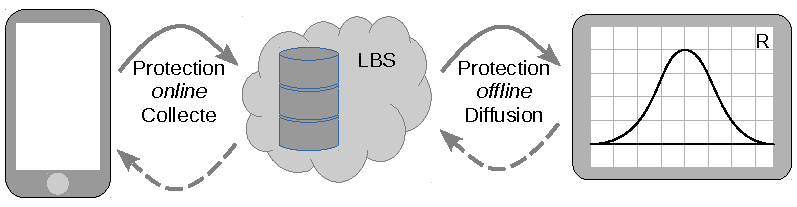
\includegraphics[scale=0.78]{Schema_phases.pdf}
%\end{center} 
On se base sur le code de \url{https://github.com/facebookresearch/pytorch-dp}\footnote{Voir \url{https://github.com/jmg-74/pytorch-dp} pour une version avec des commentaires explicatifs ajoutés.} et on analyse une exécution sur l'exemple classique du MNIST (\emph{reconnaissance de chiffres manuscrits}), fourni dans le répertoire \ttt{examples}\footnote{En pratique, il faut déplacer \ttt{mnist.py} du répertoire \ttt{examples} vers son dossier parent avant de l'exécuter.}. Celle-ci est très proche de l'utilisation sans garantie de confidentialité avec la version classique de \ttt{pytorch}, cette protection étant ajoutée explicitement lors de la phase d'entraînement, en un endroit unique dans le code.
%
\subsection{Exemple du \ttt{mnist.py}}
%
Ce dataset est traité par un CNN, \emph{Convolutional Neural Network} ou réseau de neurones convolutif, une version de réseau neuronal multicouches particulièrement adaptée au traitement des images. Avant de s'intéresser à la confidentialité différentielle, donnons la structure de base de ce réseau.\\
\textbf{\emph{Est-ce utile ? Faut-il détailler le principe d'un réseau de neurones en couches, des neurones ?}}
\begin{center}
	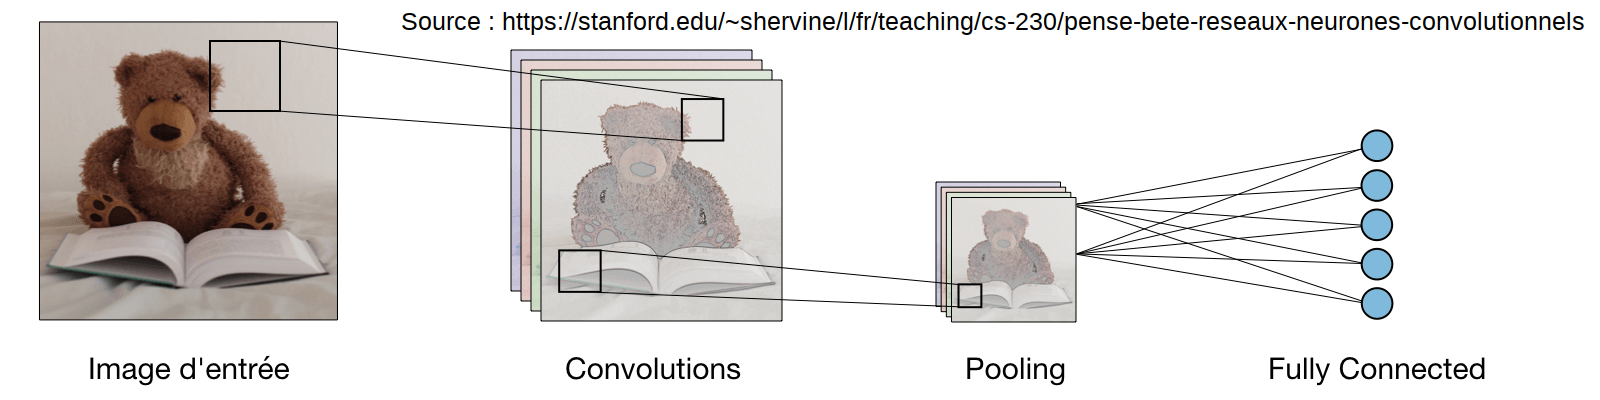
\includegraphics[width=\linewidth]{architecture-cnn.png}
\end{center}
\begin{itemize}
	\item
	Les premières couches dites convolutionnelles (\emph{convolutional layers}) donnent leur nom aux CNN. Elles ont pour but de réaliser automatiquement un pré-traitement, avec l'idée de faire apparaître des motifs exploitables dans les données de départ. On parle également de \emph{feature map} ou \emph{activation map}.\\
	En entrée on trouve la grille bidimentionnelle des pixels d'une image (la \og profondeur\fg{} ou nombre de canaux, de \emph{channels} est ici de 1 pour ces images monochromes). Un filtre (ou \emph{kernel}) constitué d'un tenseur de petite taille balaye l'image ou les données précédentes en entrée, en leur appliquant un produit terme à terme, pour produire la couche suivante en sortie. Si la profondeur est supérieure à $1$ comme ici à la deuxième étape, on additionne les valeurs obtenues pour chaque canal en entrée, associé respectivement à un canal du \emph{kernel} (on peut ajouter une éventuelle valeur constante qualifiée de biais).
	\begin{center}
		\includegraphics[width=\linewidth]{convolutions.png}
	\end{center} 
	Le script \ttt{mnist.py} s'appuie sur deux convolutions. Ainsi, le constructeur de la classe \ttt{SampleConvNet} qui hérite de \ttt{nn.Module}, définit d'abord l'attribut \ttt{conv1 = nn.Conv2d(1, 16, 8, 2)}, pour traiter $1$ canal en entrée, en produire $16$ en sortie, via un \emph{kernel} de taille $8\times8$ qui se déplace de $2$ en $2$ dans les deux dimensions de l'image à chaque étape. Puis \ttt{conv2 = nn.Conv2d(16, 32, 4, 2)} avec un filtre de $4\times4$ produisant $32$ canaux en sortie.	
	\item \textbf{\emph{FAUX, à modifier, voir forward() !!}}
	Ça n'est pas le cas ici, mais on ajoute parfois aux convolutions un \emph{pooling}, pour sous-échantillonner les données et  réduire la taille des données à traiter. Traditionnellement, on procède en remplaçant des \emph{pools} rectangulaires de pixels de petites dimensions par leur maximum ou leur moyenne, en balayant là aussi les pixels ou données en entrée. La faible taille de la couche à traiter rend ici inutile cette étape.\\
	Le décalage du \emph{pool} de pixels d'un pas au suivant (\emph{stride}, à $1$ par défaut) ainsi que la taille des marges remplies de $0$ ajoutées autour de la matrice d'entrée (\emph{padding}, par défaut à $0$) peuvent varier.
	\begin{center}
		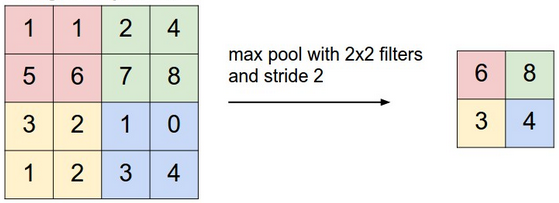
\includegraphics[width=0.7\linewidth]{pooling.png}
	\end{center}
	\item 
	On termine par les couches complètement connectées (\emph{fully connected layers}) d'un perceptron classique, une seule ici avec ses $10$ sorties associées respectivement aux chiffres à pronostiquer.
	\begin{center}
		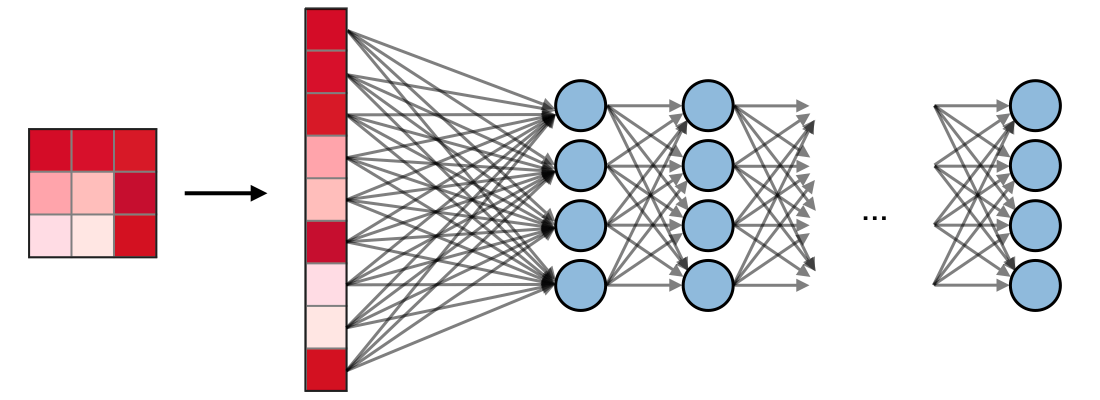
\includegraphics[width=0.8\linewidth]{fully-connected.png}
	\end{center}
   Dans le constructeur de \ttt{SampleConvNet}, l'attribut associé est \ttt{fc1 = nn.Linear(32*3*3, 10)}.\textbf{POURQUOI 3*3 ?}
 \end{itemize} 
Ce script prend en arguments entre autres \textbf{\emph{Utile (donc à compléter) ? Ou on enlève ?}}
\begin{itemize}
	\item 
	\ttt{-j} ou \ttt{--workers}, valeur par défaut $4$:  [\textbf{enlever ?}]
	\item 
	\ttt{--epochs}, valeur par défaut $90$: nombre d'\emph{epochs}, d'itérations lors de l'apprentissage par descente de gradient.
	\item 
	\ttt{-b} ou \ttt{--batch-size}, valeur par défaut $256$: taille des \emph{mini-batches}, des lots utilisés, comptée sur l'ensemble des GPU en cas de parallélisation.
	\item 
	\ttt\{--lr\} ou \textbackslash\{\}ttt\{--learning-rate\}, valeur par défaut \$0.1\$: le taux d'apprentissage, coefficient multiplicateur lors de la descente de gradient.
\end{itemize}
%
\subsection{Base \ttt{pytorch}}
%
On pourrait donner ici les grandes lignes, les principaux objets pytorch sans DP ?

%
\subsection{Organisation du code}
%
Les sources sont en \ttt{Python 3.6+} et \ttt{setup.py} à la racine assure via \code{pip install -e .} l'installation des dépendances (\emph{cf. \ttt{requirements.txt}}), ce qui a été validé sur une machine virtuelle avec une distribution \ttt{Debian 10.3} \og vierge\fg{}\footnote{on a simplement installé \ttt{git} et \ttt{pip3} (\code{apt install git pip3}) et remplacé \ttt{pip} par \ttt{pip3} pour la commande d'installation.}.

(Ajouter plutôt ici qu'on copie l'exemple à la racine du projet ?)

Le dossier \ttt{torchdp} contient le cœur du projet: 
\begin{itemize}
	\item
	\ttt{privacy\_engine.py} etc.
	\item 
	
\end{itemize}








%
\subsection{Déroulement d'une exécution}
%

\end{document}